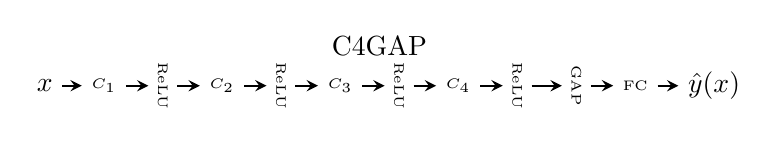
\begin{tikzpicture}

\node []  (dnn-text)at (-4.5,0.0) {C4GAP};
\node []  (dnn-output) at (-0.25,-0.5) {$\hat{y}(x)$};
\node []  (dnn-smax) at (-1.25,-0.5) {\tiny{FC}};
\draw [-stealth,thick]   (dnn-smax.east) -- (dnn-output.west);

\node [rotate=-90]  (dnn-gap) at (-2,-0.5) {\tiny{GAP}};
\draw [-stealth,thick]   (dnn-gap.north) -- (dnn-smax.west);

\node [rotate=-90] (dnn-relu-4) at (-2.75,-0.5){\tiny{ReLU}};
\node [] (dnn-c4) at (-3.5,-0.5){\tiny{$C_4$}};
\draw [-stealth,thick]   (dnn-c4.east) -- (dnn-relu-4.south);
\draw [-stealth,thick]   (dnn-relu-4.north) -- (dnn-gap.south);

\node [rotate=-90] (dnn-relu-3) at (-4.25,-0.5){\tiny{ReLU}};
\node [] (dnn-c3) at (-5,-0.5){\tiny{$C_3$}};
\draw [-stealth,thick]   (dnn-c3.east) -- (dnn-relu-3.south);
\draw [-stealth,thick]   (dnn-relu-3.north) -- (dnn-c4.west);


\node [rotate=-90] (dnn-relu-2) at (-5.75,-0.5){\tiny{ReLU}};
\node [] (dnn-c2) at (-6.5,-0.5){\tiny{$C_2$}};
\draw [-stealth,thick]   (dnn-c2.east) -- (dnn-relu-2.south);
\draw [-stealth,thick]   (dnn-relu-2.north) -- (dnn-c3.west);

\node [rotate=-90] (dnn-relu-1) at (-7.25,-0.5){\tiny{ReLU}};
\node [] (dnn-c1) at (-8,-0.5){\tiny{$C_1$}};
\draw [-stealth,thick]   (dnn-c1.east) -- (dnn-relu-1.south);
\draw [-stealth,thick]   (dnn-relu-1.north) -- (dnn-c2.west);



\node [] (dnn-input) at (-8.75,-0.5){$x$};
\draw [-stealth,thick]   (dnn-input.east) -- (dnn-c1.west);

\node []  (dummy)at (-4.5,-1) {};

%%%%%%%%%%%%%%%%%%%%%%%%%%%%%%%%%%%%%%%%%%%%%%%%%%%%%%%%%%%%%%%%%

	
\end{tikzpicture}

